
Este capítulo apresenta a metodologia aplicada para realizar o presente trabalho. Para isso, foram definidas três grandes etapas (Figura~\ref{fig:fluxogramaMetodologia}): i) pesquisa bibliográfica na qual são analisadas tecnologias variadas relevantes ao contexto do trabalho, ii) modelagem da solução na qual o robô simulado é desenvolvido, iii) validação final do modelo completamente integrado com análise do resultado. 

\begin{figure}[H]
    \centering
    \caption{Fluxograma das etapas da metodologia}
    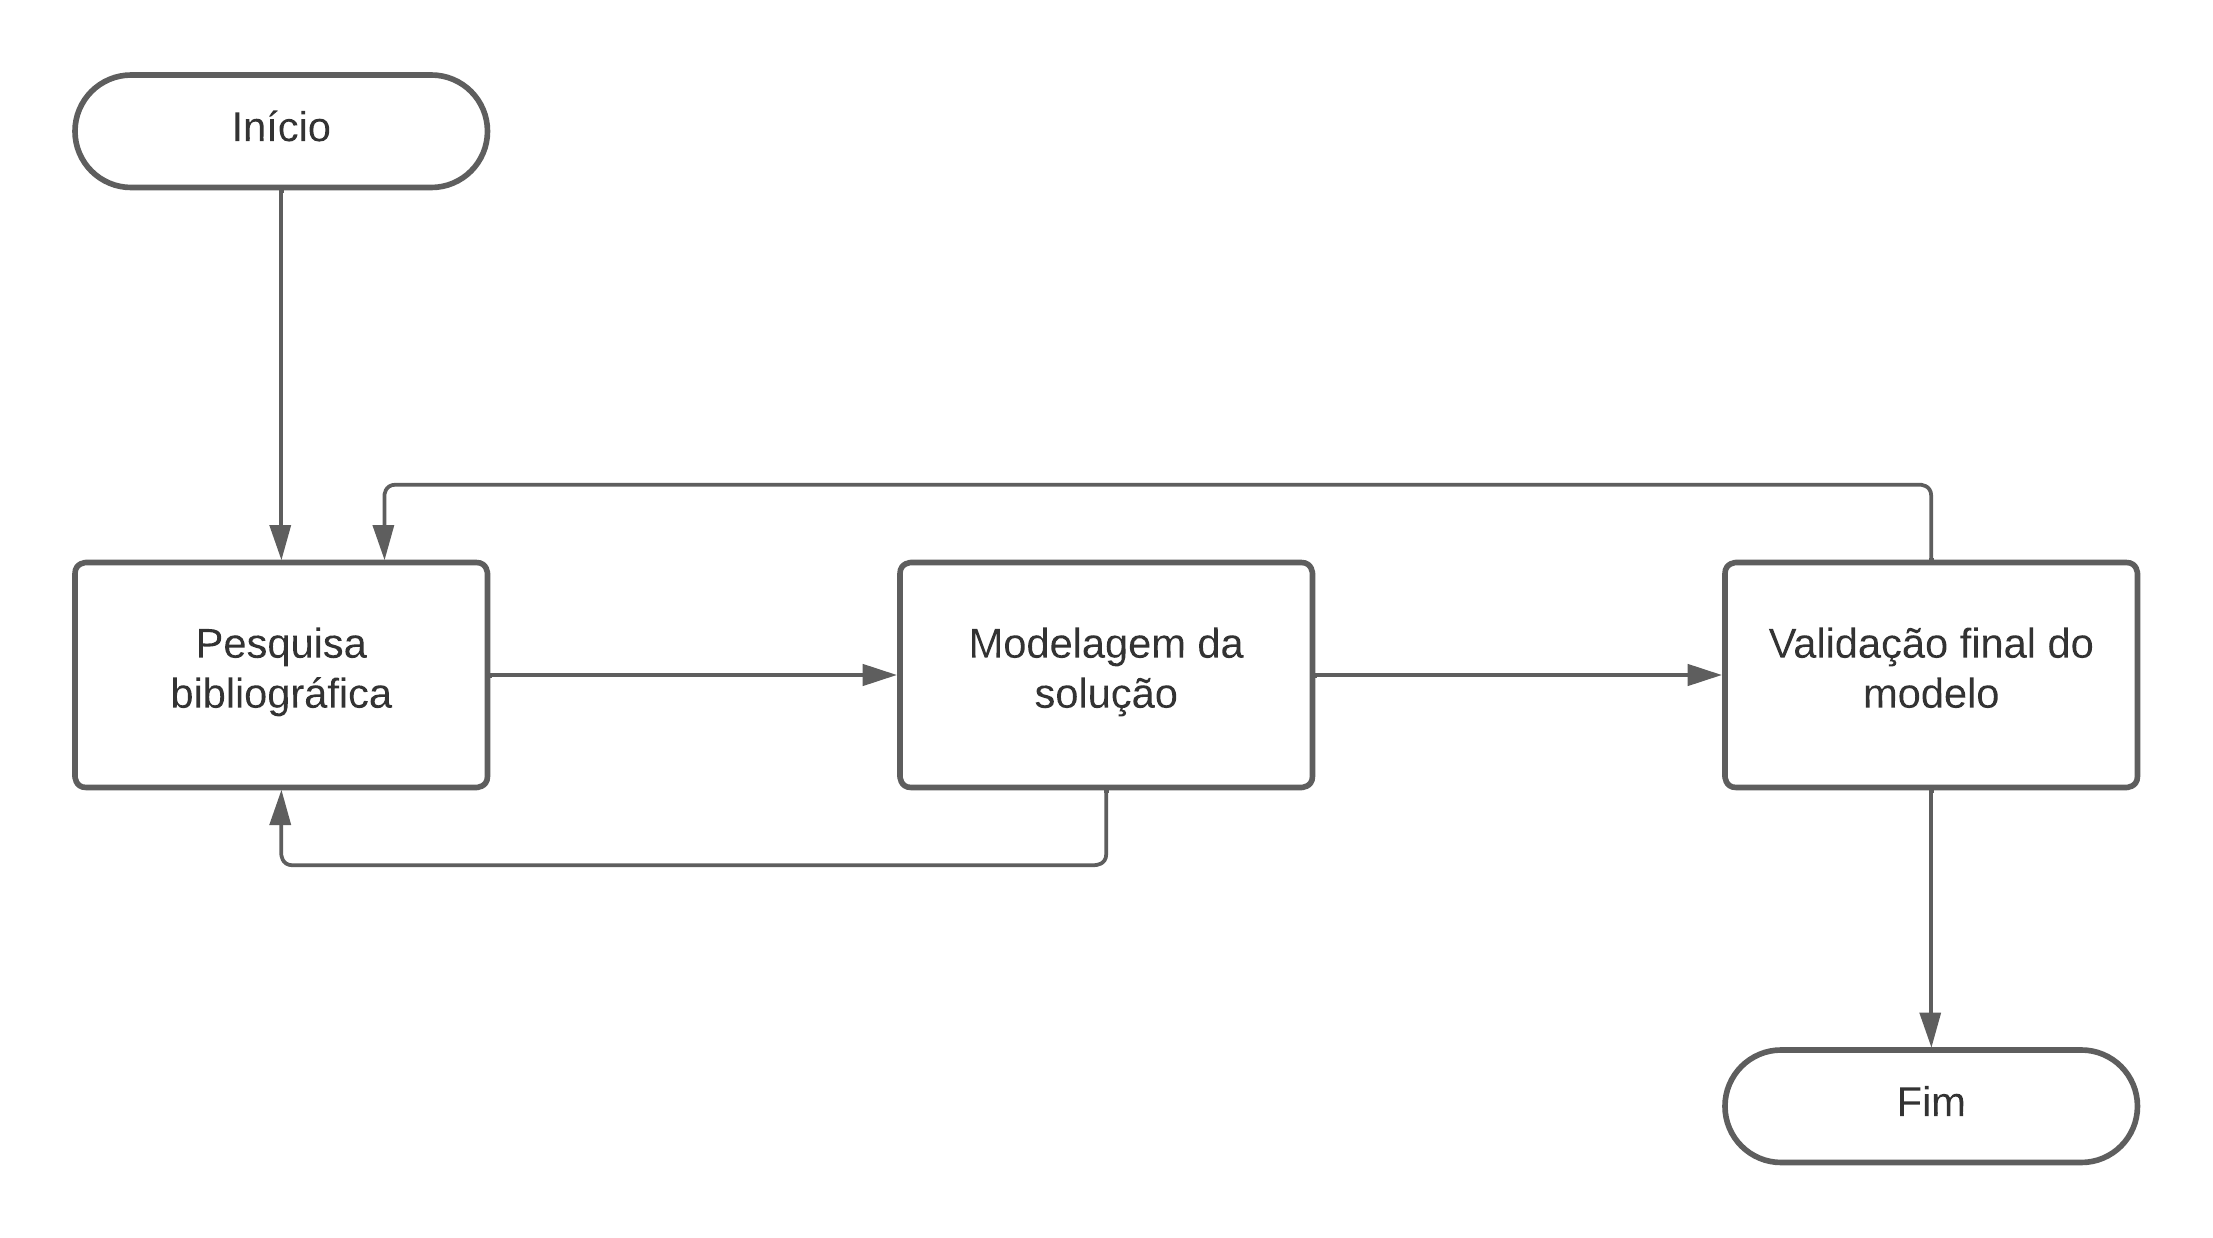
\includegraphics[scale=0.8]{fluxogramaMetodologia.png}
    \caption*{Fonte: Autora (2023).}
    \label{fig:fluxogramaMetodologia}
\end{figure}

A metodologia desempenhada no referente trabalho foi baseada na abordagem de \textit{Design Science Research} (DSR). Essa, por sua vez, é aplicada em pesquisas que almejam produzir um artefato (como um modelo ou uma aplicação) para solucionar um problema relevante \cite{dsrBook:2015}. A pesquisa deste trabalho cumpre as orientações para uma pesquisa de \textit{Design Science}, dispostas por \citet{dsrIS:2004}, reforçando como esta metodologia é apropriada para este trabalho. 

Assim, conforme os critérios da DSR, este trabalho visa produzir um artefato viável a partir do modelo a ser proposto para resolver o problema de desenvolvimento de robôs de serviço doméstico disposto anteriormente. Além de contribuir para a pesquisa de implementação de tecnologias para: a navegação autônoma e simulação robótica. Também, possui métodos específicos para a construção do modelo (seguindo a abordagem incremental de desenvolvimento de \textit{software}) e sua validação (utilizando casos de teste).

Para \citet{dsrBook:2015}, a metodologia DSR propõe uma pesquisa com 12 etapas, nas quais o problema a ser resolvido é identificado, as suas teorias e conceitos são estudados a partir de uma pesquisa bibliográfica e os artefatos semelhantes, para a solução do problema em questão, são constatados. Com isso, o artefato é desenvolvido e validado. Por fim, o resultado obtido é analisado e as conclusões são divulgadas para contribuir na área de pesquisa. Portanto, as três grandes etapas (Figura~\ref{fig:fluxogramaMetodologia}) a serem conduzidas neste trabalho se baseiam nesse fluxo de atividades proposto pelo DSR.

\section{Etapa de Pesquisa Bibliográfica}
A fim de desenvolver um robô autônomo móvel com as tecnologias mais adequadas e relevantes atualmente, foram realizadas duas pesquisas bibliográficas específicas. Essas pesquisas buscam identificar quais são as tecnologias mais utilizadas ao implementar a localização de um robô autônomo móvel, principalmente as abordagens utilizadas e os instrumentos de percepção do ambiente integrados.

Essas pesquisas bibliográficas específicas foram realizadas através do método de revisão da literatura narrativa com o uso de algumas características chaves da revisão sistemática. A fim de obter resultados mais imparciais e replicáveis, foram utilizados aspectos importantes da revisão sistemática dispostos em \citet{revisaoSistematica}, sendo eles: i) uma declaração explícita das perguntas a serem respondidas; ii) uma sequência de palavras-chave para cada pesquisa específica; iii) critérios de inclusão e exclusão para a filtragem dos artigos obtidos pelas buscas. 

Optou-se por realizar uma revisão narrativa por permitir uma compreensão do contexto de forma maleável \cite{revisaoNarrativa}. Visto que o objetivo das pesquisas bibliográficas mencionadas é compreender esse contexto geral dos temas supracitados para a tomada de decisão do uso das tecnologias mais relevantes e adequadas, foi identificado que a revisão sistemática não se encaixa. Isso se dá principalmente porque esse formato de revisão implica em uma análise detalhada de todos os dados obtidos em cada publicação acadêmica selecionada pela busca, além de requisitar uma sintetização dessas publicações, ou seja, informações desnecessárias para o alvo das pesquisas \cite{revisaoSistematica, literaturas}. Outro fator que impossibilita o uso da revisão sistemática é a exigência de pelo menos mais de um autor para tentar garantir o maior nível de imparcialidade possível \cite{revisaoSistematica, literaturas}.

Para encontrar os materiais acadêmicos relevantes foram utilizados os repositórios IEEE Xplore e ACM Digital Library, por serem específicos das áreas das Engenharias e da Computação. Além disso, foram definidas sequências de palavras-chave em inglês para buscar nos repositórios. Para focar a análise dos materiais, foram estabelecidos critérios de inclusão e exclusão para cada busca, filtrando os materiais com maior relevância para o assunto. 

Foi realizada uma sequência de pesquisas para identificar as tecnologias mais relevantes para localização do robô e percepção do ambiente. Primeiramente, foi efetuada a pesquisa para responder a pergunta: qual a abordagem mais utilizada para a localização de robôs autônomos móveis domésticos? Para isso, a busca foi realizada com a seguinte sequência de palavras-chave: 'autonomous mobile robot localization algorithms'. 

Com a resposta da pergunta inicial anterior, foi realizada a segunda pesquisa bibliográfica específica para responder outra pergunta: qual o instrumento mais utilizado para a percepção de um ambiente interno para um robô autônomo móvel que se localiza pela abordagem SLAM? Para essa segunda pesquisa, foi utilizada outra sequência de palavras-chave: 'slam sensing mobile robot'. Para ambas as buscas, foi utilizado o operador lógico AND entre cada palavra-chave, a fim de obter resultados mais específicos para os temas.

Em ambas as pesquisas bibliográficas específicas, foi realizada uma análise nos títulos e resumos dos artigos encontrados, para filtrar as publicações que não se encaixavam no escopo, seguindo as delimitações dos critérios de inclusão e exclusão, expostos na Tabela \ref{tab:prompts}. Os materiais foram filtrados com o apoio da plataforma Rayyan que disponibiliza uma estrutura para analisar artigos de uma forma mais eficiente \cite{rayyan}. 

\begin{table}[H]
\caption{Critérios de inclusão e exclusão}
\label{tab:prompts}
\resizebox{\textwidth}{!}{%
\begin{tabular}{p{7cm}|p{7cm}}
  \multicolumn{1}{c|}{\textbf{Inclusão}} &
  \multicolumn{1}{c}{\textbf{Exclusão}} \\ \hline
\begin{itemize}
    \item Aplicado em robótica móvel;
    \item Aplicado para ambiente interno doméstico;
    \item Escrito em inglês, espanhol ou português.
\end{itemize}&
\begin{itemize}
   \item Aplicado em navegação externa, água, aérea, indústria ou ambiente externo;
    \item Relacionado à realidade aumentada;
    \item Aplicado para veículos, drones, enxames de drones, múltiplo-robôs;
    \item Com necessidade de rede local, internet, wi-fi;
    \item Fora do escopo de robôs;
    \item Escrito em outro idioma que não seja inglês, espanhol ou português.
\end{itemize}% \\ \hline
\end{tabular}
%
}
\caption*{Fonte: Autora (2023).}
\end{table}

Dito isso, ambas pesquisas bibliográficas passaram por quatro momentos específicos, sendo eles:
\begin{itemize}
    \item Momento 1: Busca dos materiais acadêmicos nos repositórios com as palavras-chave definidas;
    \item Momento 2: Descarte dos materiais, resultantes da busca, que não pertencem ao período de 2018 a 2023;
    \item Momento 3: Descarte dos materiais, resultantes do momento anterior, que não são artigos publicados em periódicos;
    \item Momento 4: Descarte dos artigos, resultantes do momento anterior, que não cumprem os critérios de inclusão e/ou contém os critérios de exclusão.
\end{itemize}

Após a filtragem dos materiais encontrados na busca, foram identificados as tecnologias utilizadas em cada pesquisa, no intuito de encontrar qual delas é a predominante, e consequentemente, a mais relevante para os temas levantados.

\section{Etapa de Modelagem da Solução}
A modelagem foi realizada conforme os princípios da metodologia incremental de desenvolvimento de software. A abordagem incremental, de acordo com \citet{softwareSommerville:2011}, permite a implementação de funcionalidades essenciais em uma primeira versão e integrar outras funcionalidades a cada nova versão até que o sistema adequado seja desenvolvido conforme os requisitos levantados. 

Seguindo a metodologia incremental, em cada versão foram realizados o desenvolvimento e validação das novas funcionalidades. Esse ciclo de implementação tem o intuito de analisar se os requisitos levantados estão sendo alcançados corretamente, identificar falhas com antecedência e ajustar as funcionalidades antes de tornar o sistema mais complexo. 

\section{Etapa de Validação Final}
Com o modelo proposto completamente integrado, o mesmo foi conduzido por um processo de validação final de modo a analisar a adequação da proposta perante as especificações identificadas. Para isso, foram realizados testes de caixa preta conforme uma série de casos de testes definidos.

Os casos de teste são cenários que especificam uma entrada ou uma ação para os teste, além de um resultado esperado \cite{testes}. Para a validação do modelo proposto foram elaborados casos de teste baseados nos requisitos funcionais e não funcionais do robô e do ambiente simulados. O intuito dessa validação pelos casos de teste é identificar o comportamento do modelo proposto conforme as circunstâncias definidas previamente. Além disso, possibilita quantificar a adequação da solução proposta perante os requisitos identificados para o problema norteante da pesquisa. 

Os testes efetuados conforme os cenários especificados, utilizaram a técnica de testes de caixa preta, os quais visam verificar as funcionalidades específicas do sistema em alto nível \cite{testes}. Ademais, para os requisitos funcionais do robô, foi optado por realizar cinco repetições para cada caso de teste. Essas repetições têm o intuito de obter uma média de acertos perante os resultados esperados, visto que a execução do sistema pode encontrar instabilidades, mesmo sendo por simulação. Por fim, os resultados dos casos de teste foram classificados em 1) bem sucedidos, no qual o comportamento desejado foi obtido segundo a ação detalhada, e 2) não sucedido, caso o contrário. Os casos de teste com repetições foram considerados bem sucedidos se, e somente se, obtivessem uma porcentagem de sucesso maior que 50\%.

A fim de discernir as diferenças e similaridades entre o presente trabalho e as pesquisas correlatas que aplicam abordagens semelhantes para o desenvolvimento de um robô autônomo móvel, foi realizada uma análise comparativa. Essa análise consistiu em comparar os resultados,  expostos em trabalhos correlatos, sobre a implementação da navegação autônoma do robô móvel e do desenvolvimento em perspectiva geral.


